\documentclass{beamer}
\usepackage{kotex}
%\usetheme{Warsaw}
\usetheme{metropolis} % Metropolis theme is modern and minimalistic
%\usetheme{Madrid} % Fee6l free to change the theme
%\usetheme{Berkeley}

\usepackage{commath}

% Define custom colors (choose colors that suit your style)
\definecolor{PrimaryColor}{RGB}{36, 123, 160}
\definecolor{SecondaryColor}{RGB}{112, 193, 179}

\setbeamercolor{palette primary}{bg=PrimaryColor,fg=white}
\setbeamercolor{palette secondary}{bg=SecondaryColor,fg=white}

% Add any packages you need here
\usepackage{graphicx}
\usepackage{booktabs}
\usepackage{tabularx}
\usepackage{multirow}
\usepackage{tikz}
\usepackage{hyperref}

\usepackage[ruled,linesnumbered]{algorithm2e}
\usepackage{setspace}
\usepackage{algpseudocode}
\SetKwComment{Comment}{/* }{ */}
\SetKw{Break}{break}
\SetKw{Downto}{downto}
\SetKwProg{Fn}{Function}{:}{end}
\SetKwProg{Procedure}{procedure}{:}{end}
\SetKwProg{Construct}{Construct}{:}{end}
\SetKwFunction{KeyGen}{KeyGen}

\newcommand{\Z}{\mathbb{Z}}
\newcommand{\of}[1]{\left( #1 \right)} 

\title[Short Title]{PUBAO - Over the Long Long}
\subtitle{Project: P.A.N.D.A.'s Unbounded Big Arithmetic Operations}
\author{Team: Programmers Aspiring to Navigate Digital Arithmetic (P.A.N.D.A)}
\institute{국민대학교 과학기술대학 정보보안암호수학과}
\date{\today}

\logo{
\includegraphics[height=1cm]{PANDA_logo.png}}


\begin{document}
	
	\begin{frame}
		\titlepage
	\end{frame}
	
	\begin{frame}{목차}
		\tableofcontents
	\end{frame}

\section{I. 개발자들아, 나와라!}

\begin{frame}{I.1 개발진 소개}
	% Use two columns: one for photos and one for text
	\begin{columns}
		\column{0.4\textwidth}
%		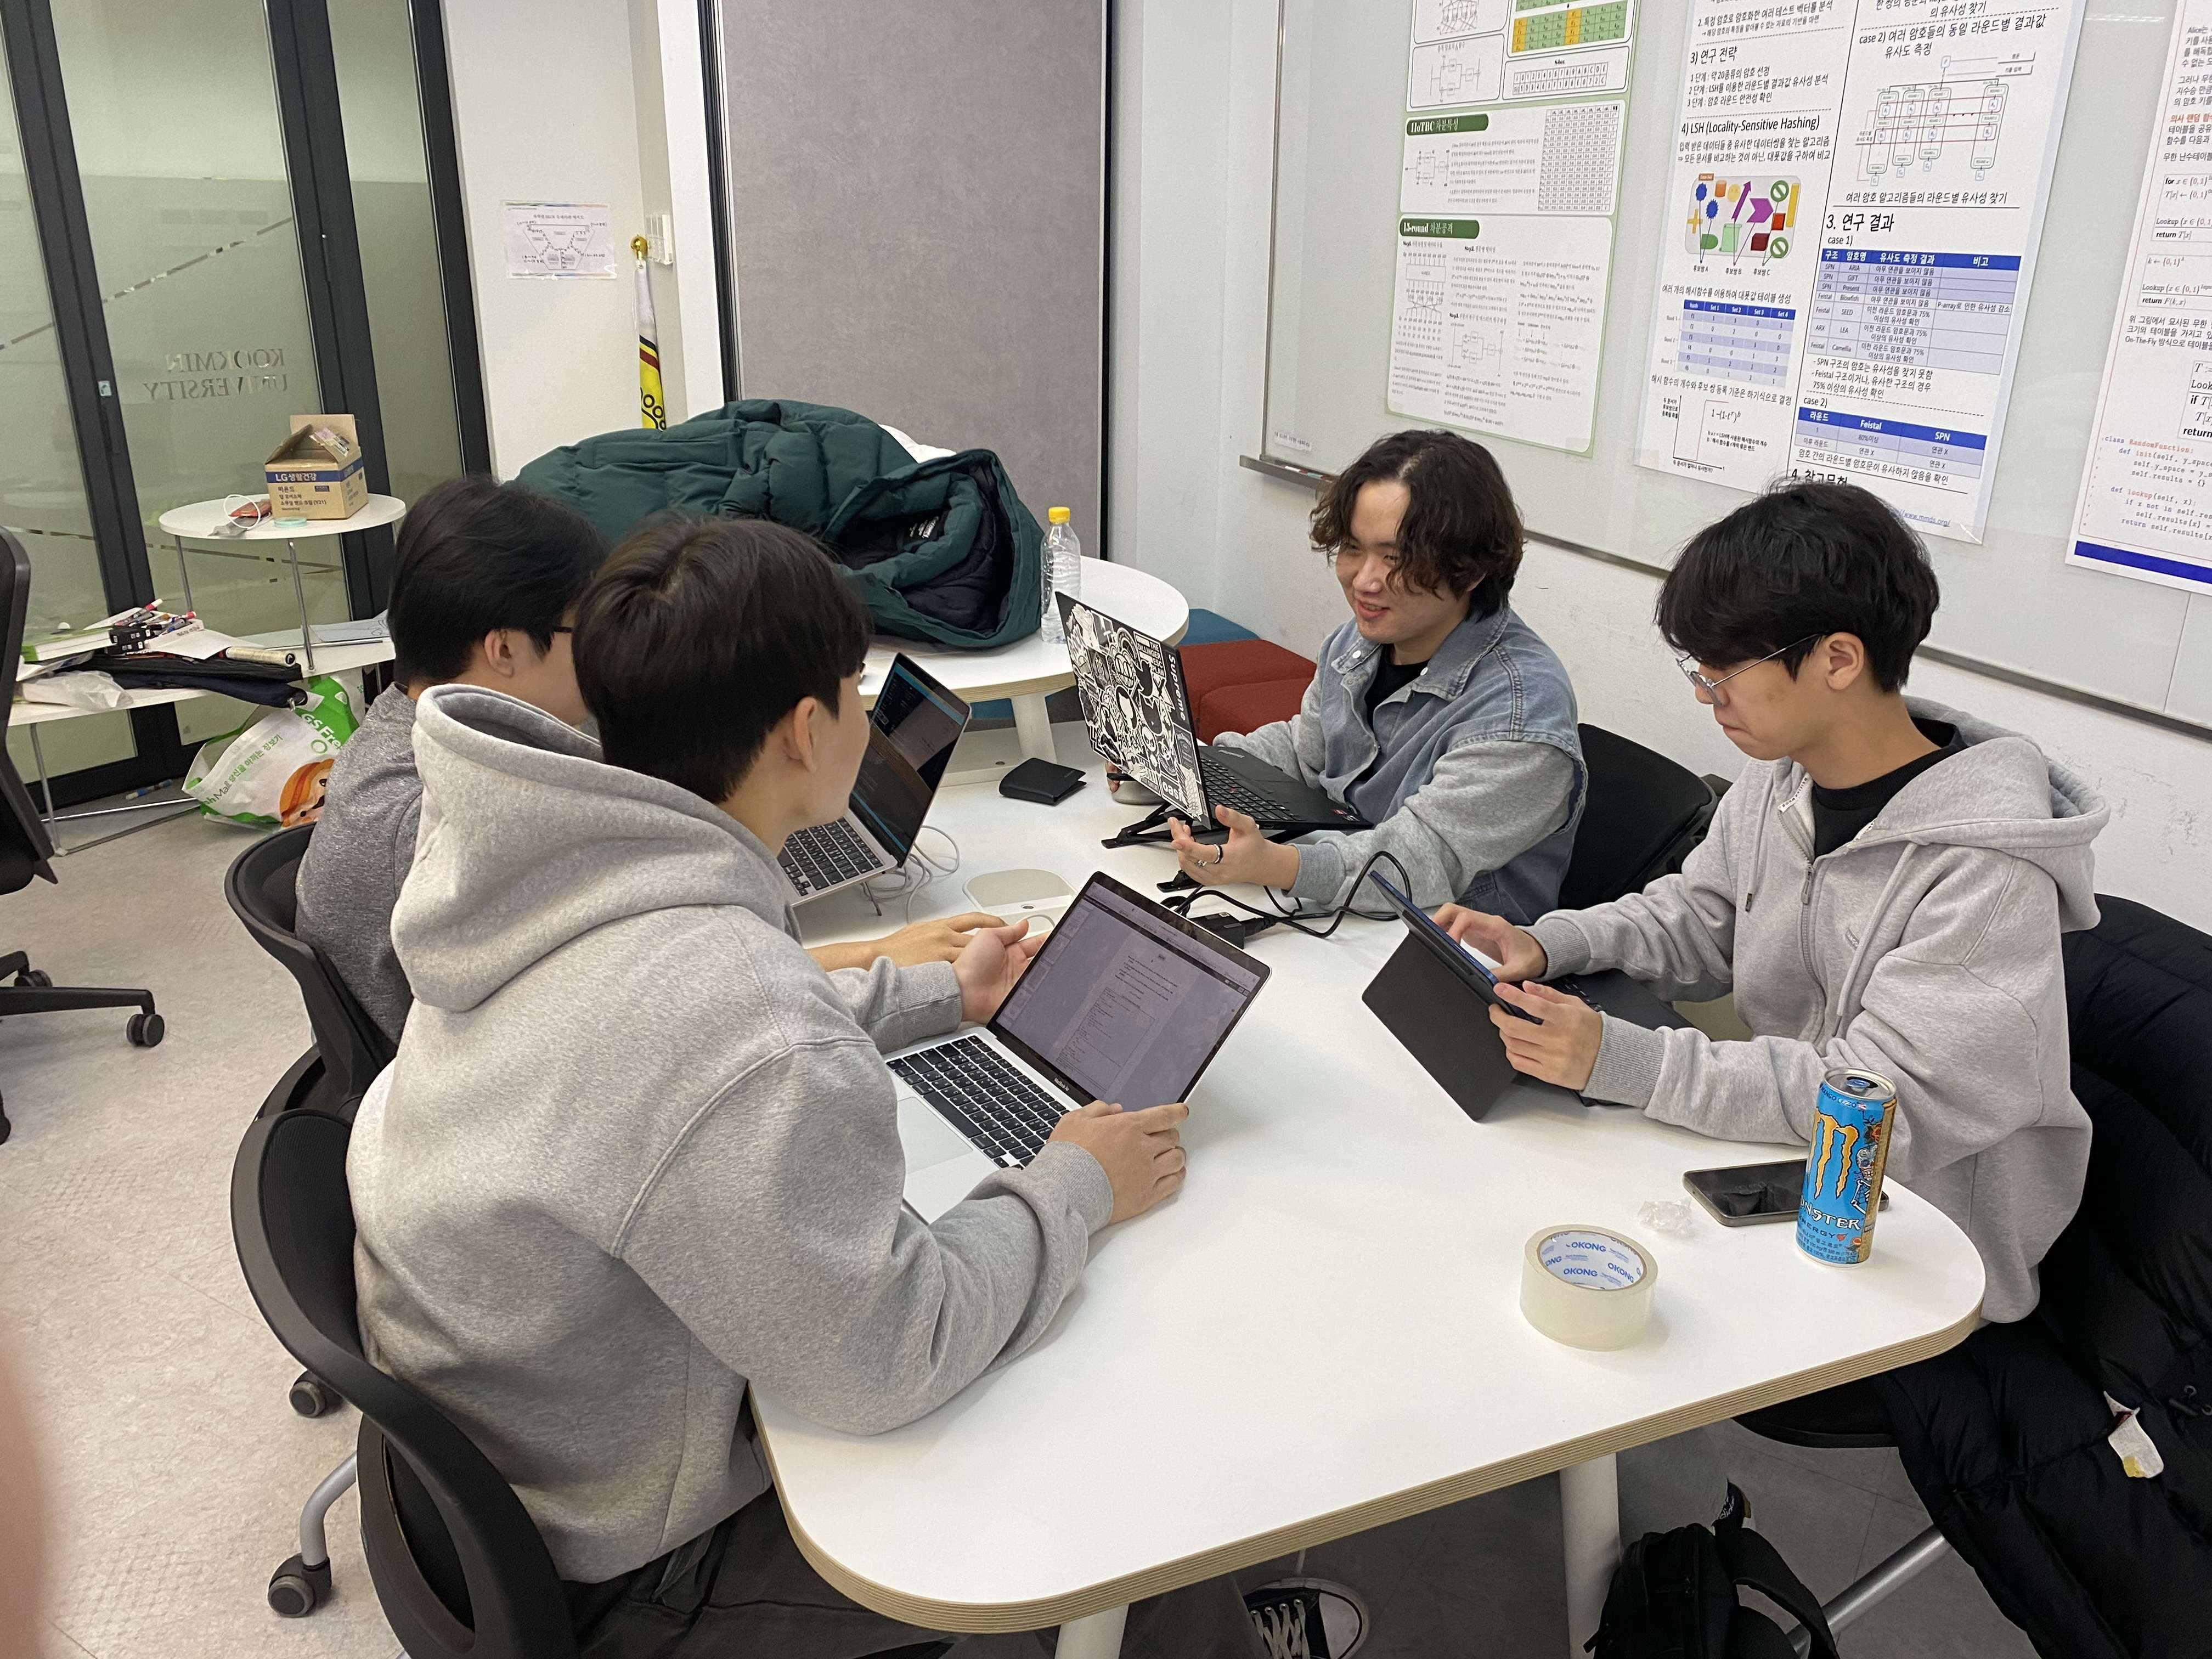
\includegraphics[width=\textwidth]{team_photo.jpg}
		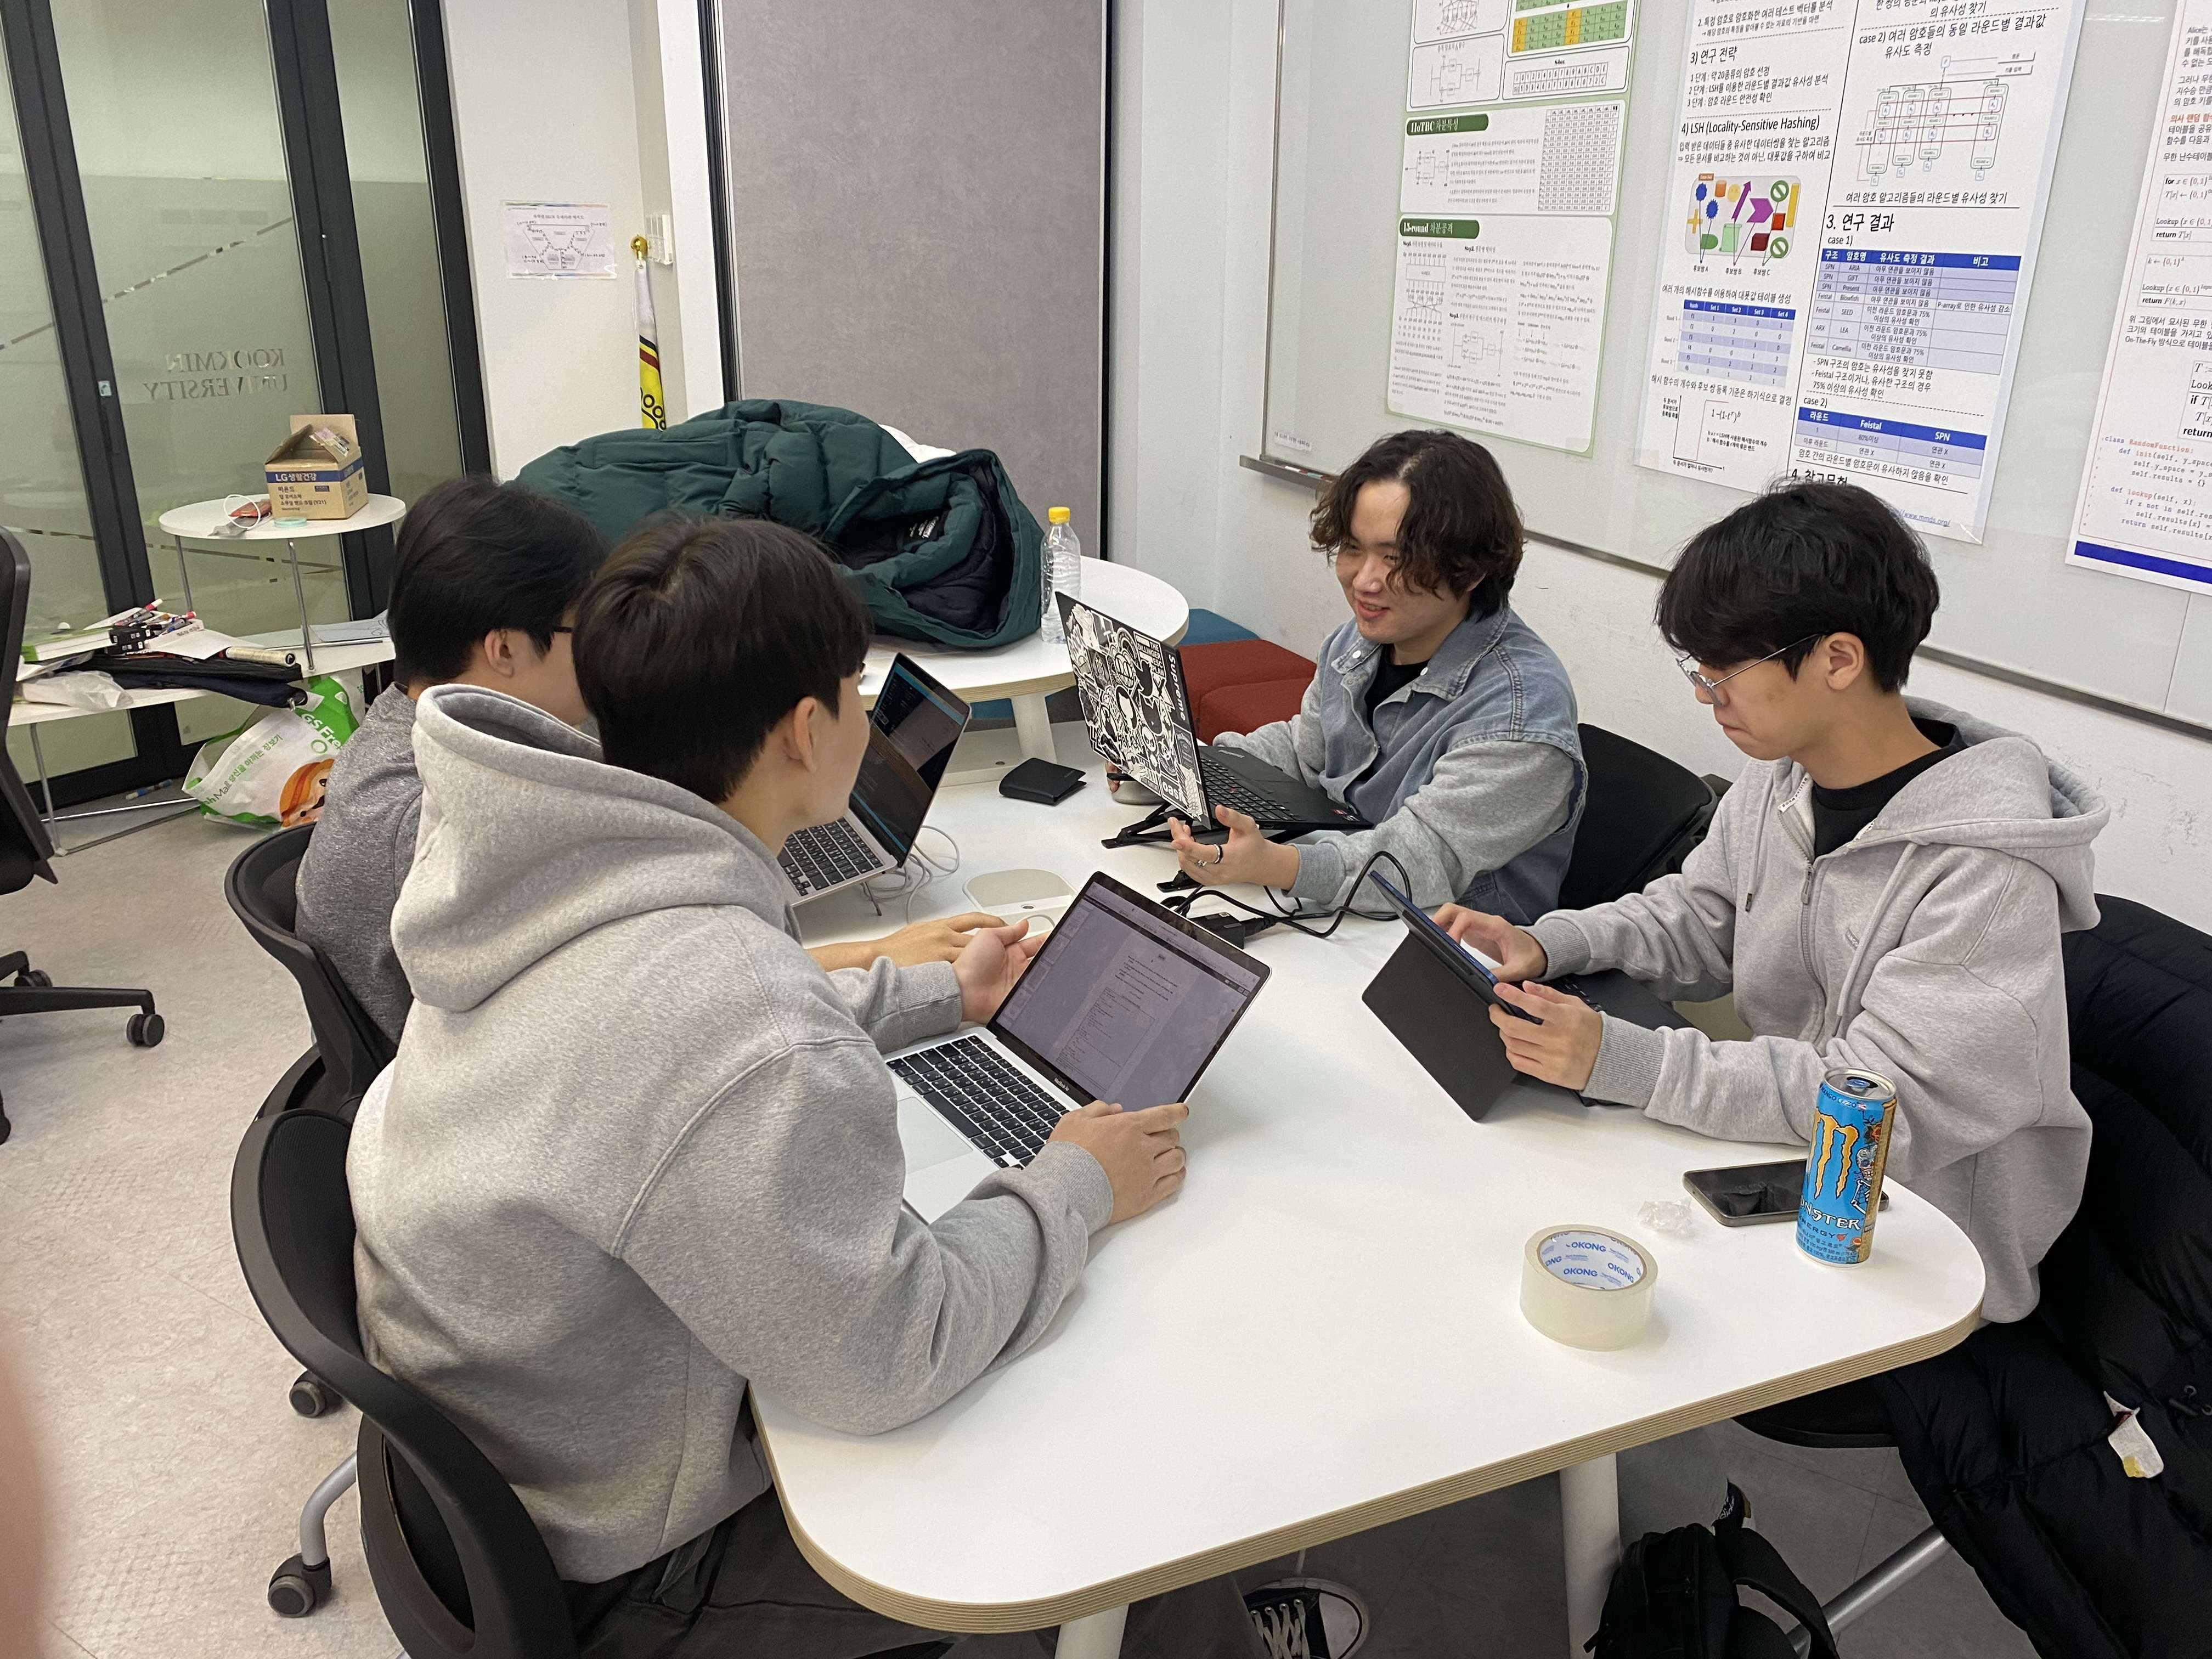
\includegraphics[scale=.035]{team_photo.jpg}
		\column{0.5\textwidth}
		% List your team members and roles here
		\begin{itemize}
			\item 지용현(20192250, Leader)
			\item 문예찬(20192230, Builder)
			\item 김예찬(20192220, Validator)
			\item 유근오(20232093, Intern)
			% Add more members as needed
		\end{itemize}
	\end{columns}
\end{frame}

\begin{frame}{I.2 팀원 소개}
	\begin{columns}[T,onlytextwidth]
		\column{0.5\textwidth}
		\centering
		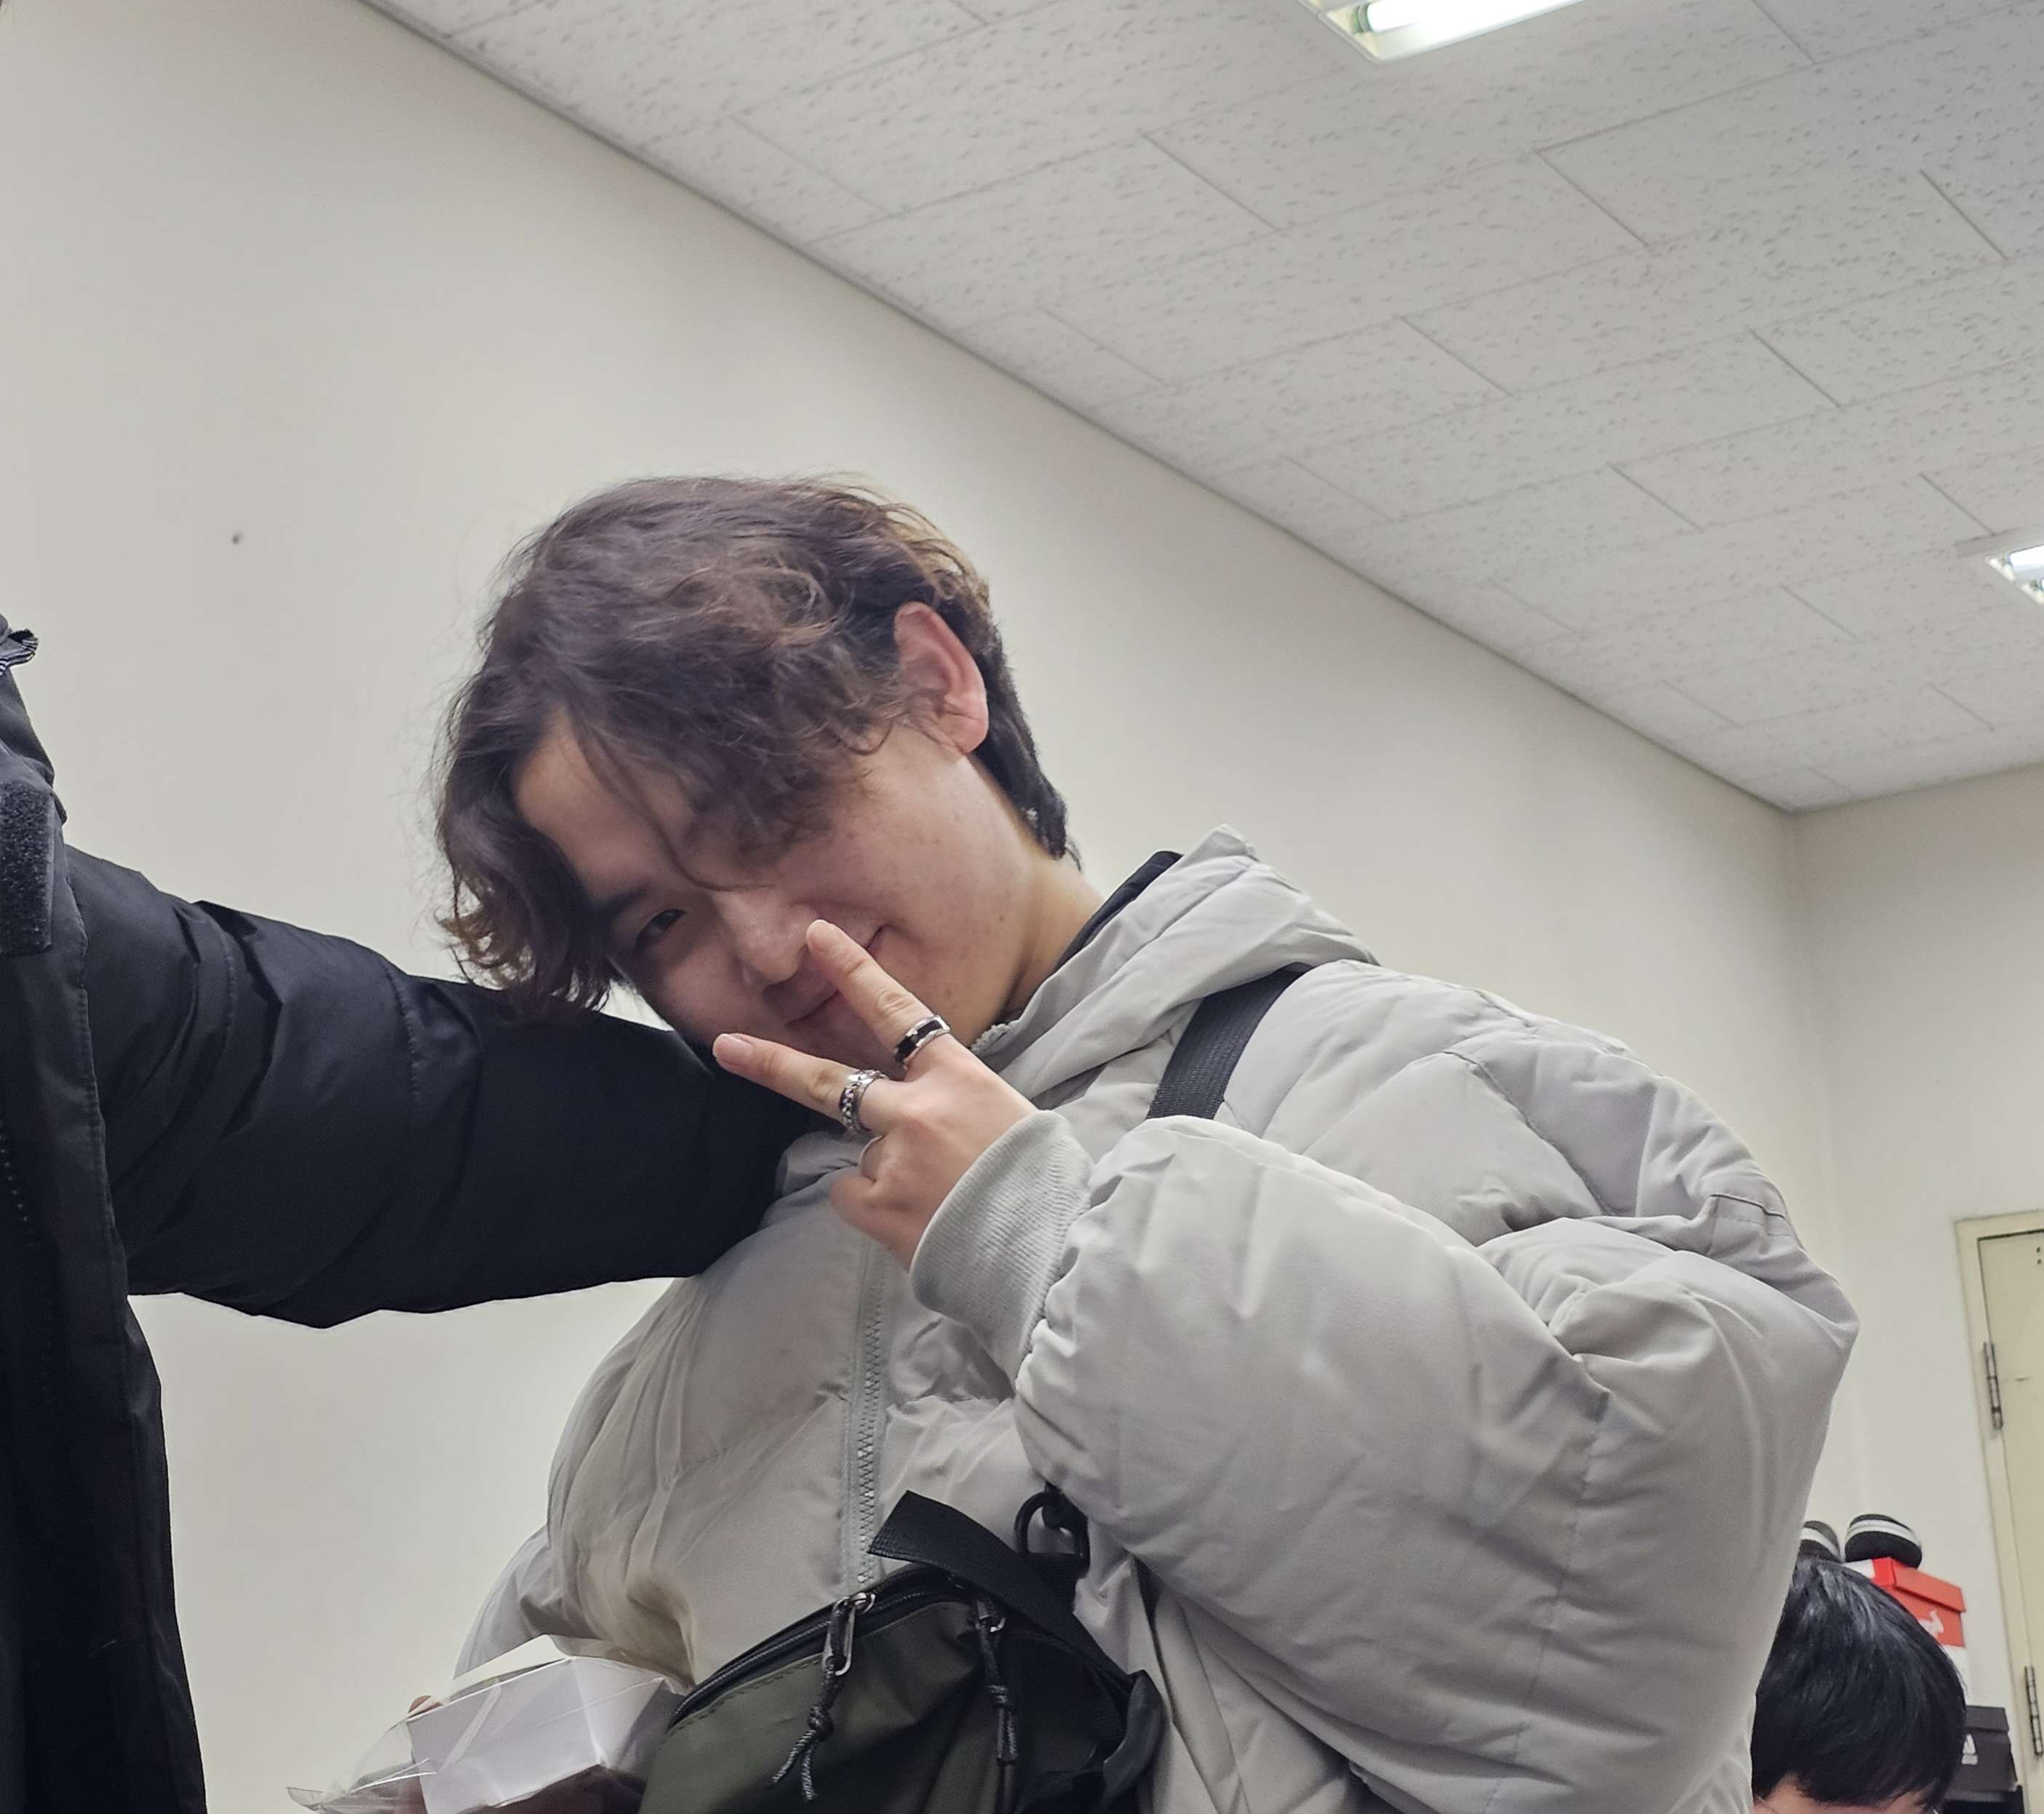
\includegraphics[width=.5\linewidth,height=.35\textheight]{ji.jpg}\\
		\textbf{지용현 (Leader)}\\
		\textit{``위대한 리더''}\\
		\begin{flushleft}\footnotesize
			특징: 전국민초사랑연맹 임원\\
			한마디: \textbf{버그가 아니라 이스터에그다}
		\end{flushleft}
		
		\column{0.5\textwidth}
		\centering
		
\includegraphics[width=.5\linewidth,height=.35\textheight]{yoo.jpg}\\
		\textbf{유근오 (Intern)}\\
		\textit{``꿈꾸는 샛별''}\\
		\begin{flushleft}\footnotesize
			특징: 집돌이\\
			한마디: \textbf{코딩은 실수를 찾고 숨기는 과정}
		\end{flushleft}
	\end{columns}
\end{frame}
\begin{frame}{I.2 팀원 소개}
	\begin{columns}[T,onlytextwidth]	
		\column{0.48\textwidth}
		\centering
		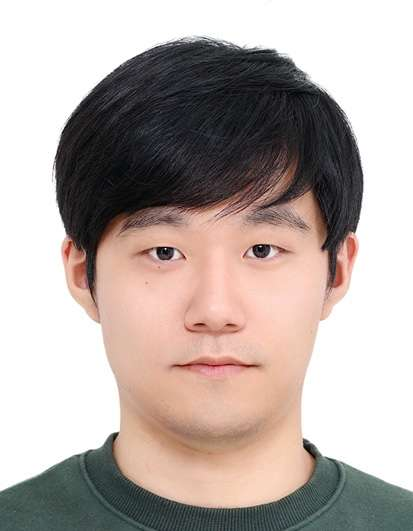
\includegraphics[width=.5\linewidth,height=.35\textheight]{moon.jpg}\\
		\textbf{문예찬 (Builder)}\\
		\textit{``창조의 손길''}\\
		\begin{flushleft}\footnotesize
			특징: 목 디스크, 허리디스크\\
			한마디: \textbf{적당한 알콜은 코딩을 도운다.}
		\end{flushleft}
	
		\column{0.48\textwidth}
		\centering
		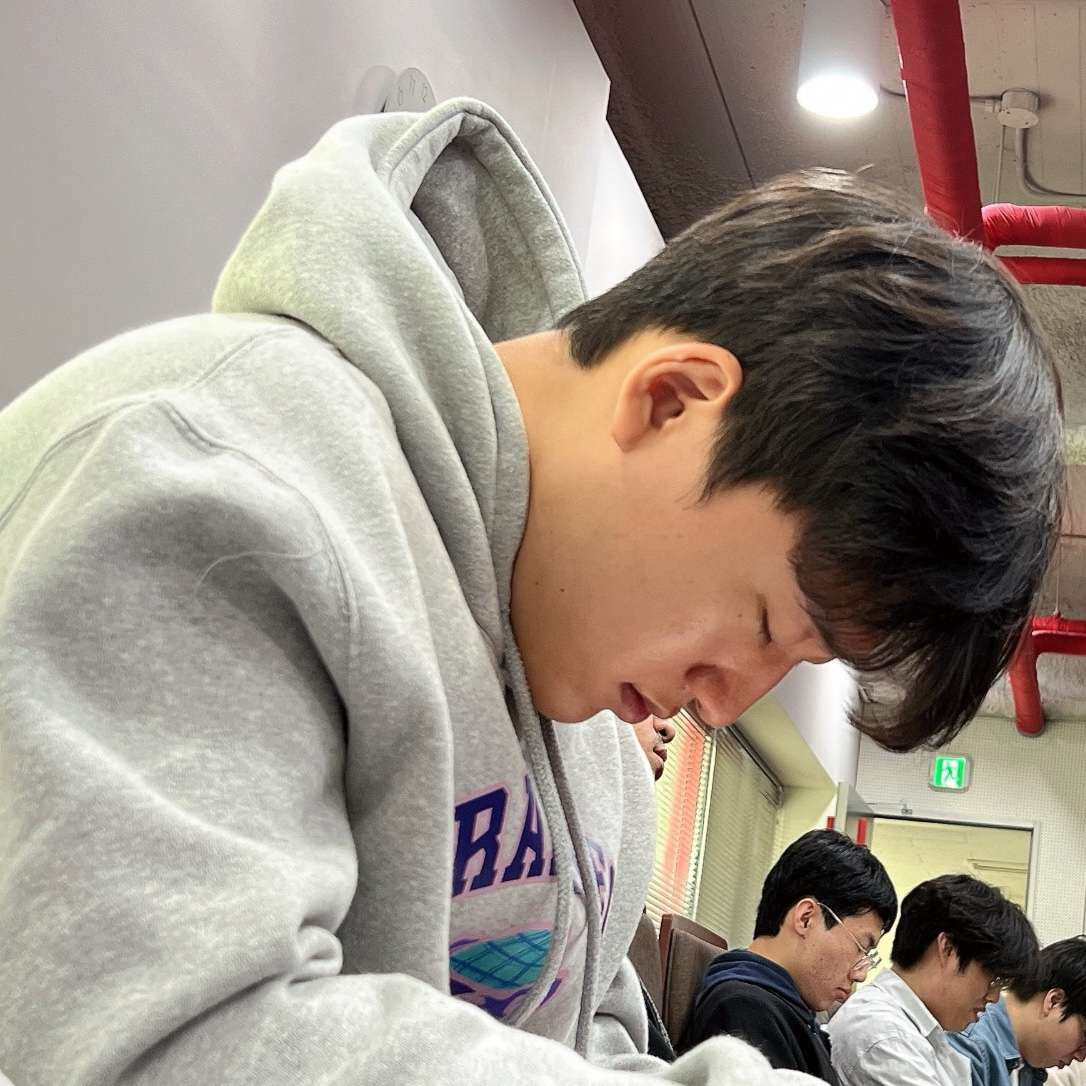
\includegraphics[width=.5\linewidth,height=.35\textheight]{kim.jpg}\\
		\textbf{김예찬 (Vaildator)}\\
		\textit{``오류 저격수''}\\
		\begin{flushleft}\footnotesize
			특징: 앱등이, 잠꾸러기\\
			한마디: \textbf{ 적당한 코딩은 알콜을 부른다.}
		\end{flushleft}
	\end{columns}
\end{frame}
\section{II. 전략은 우리의 무기!}
\begin{frame}{II.1 개발 목표}
	\begin{itemize}[<+->]
		\item 큰 정수에 대한 연산을 처리할 수 있는 라이브러리를 개발. \[
		a\pm b=?\quad a*b=?\quad a/b=?\quad a \bmod b=?\quad a^b\bmod{c}=?
		\]
		\item 라이브러리를 통한 BSGS 알고리즘으로 DLP 해독기 개발. \[
		g^x\equiv h\ (\bmod{n})\implies x=?
		\]
		% and so on
	\end{itemize}
\end{frame}
\begin{frame}
	\frametitle{II.2 개발 전략 - Notion을 통한 협업}
	\alert{\bf Notion을 활용한 협업 활동}\\
	\ \\
	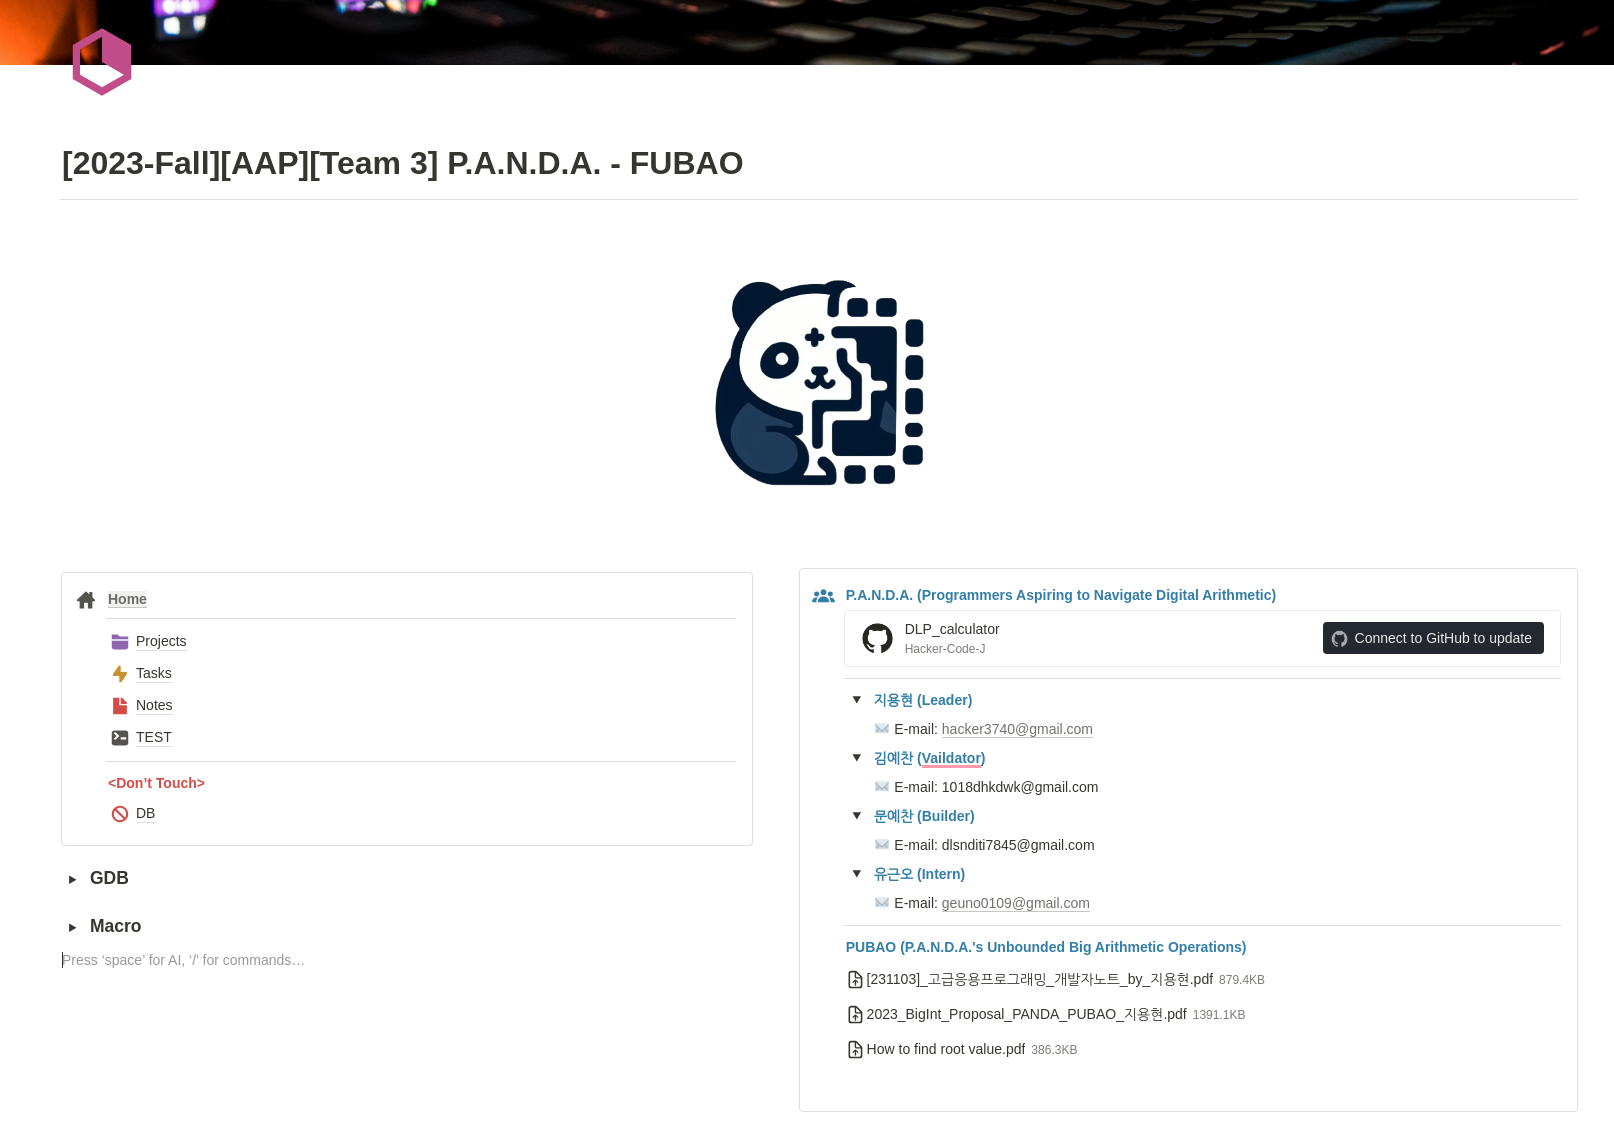
\includegraphics[width=\linewidth,height=.825\textheight]{notion1.png}\\
\end{frame}
\begin{frame}
	\frametitle{II.2 개발 전략 - Notion을 통한 협업}
	\alert{\bf 브레인스토밍}\\
	\ \\
	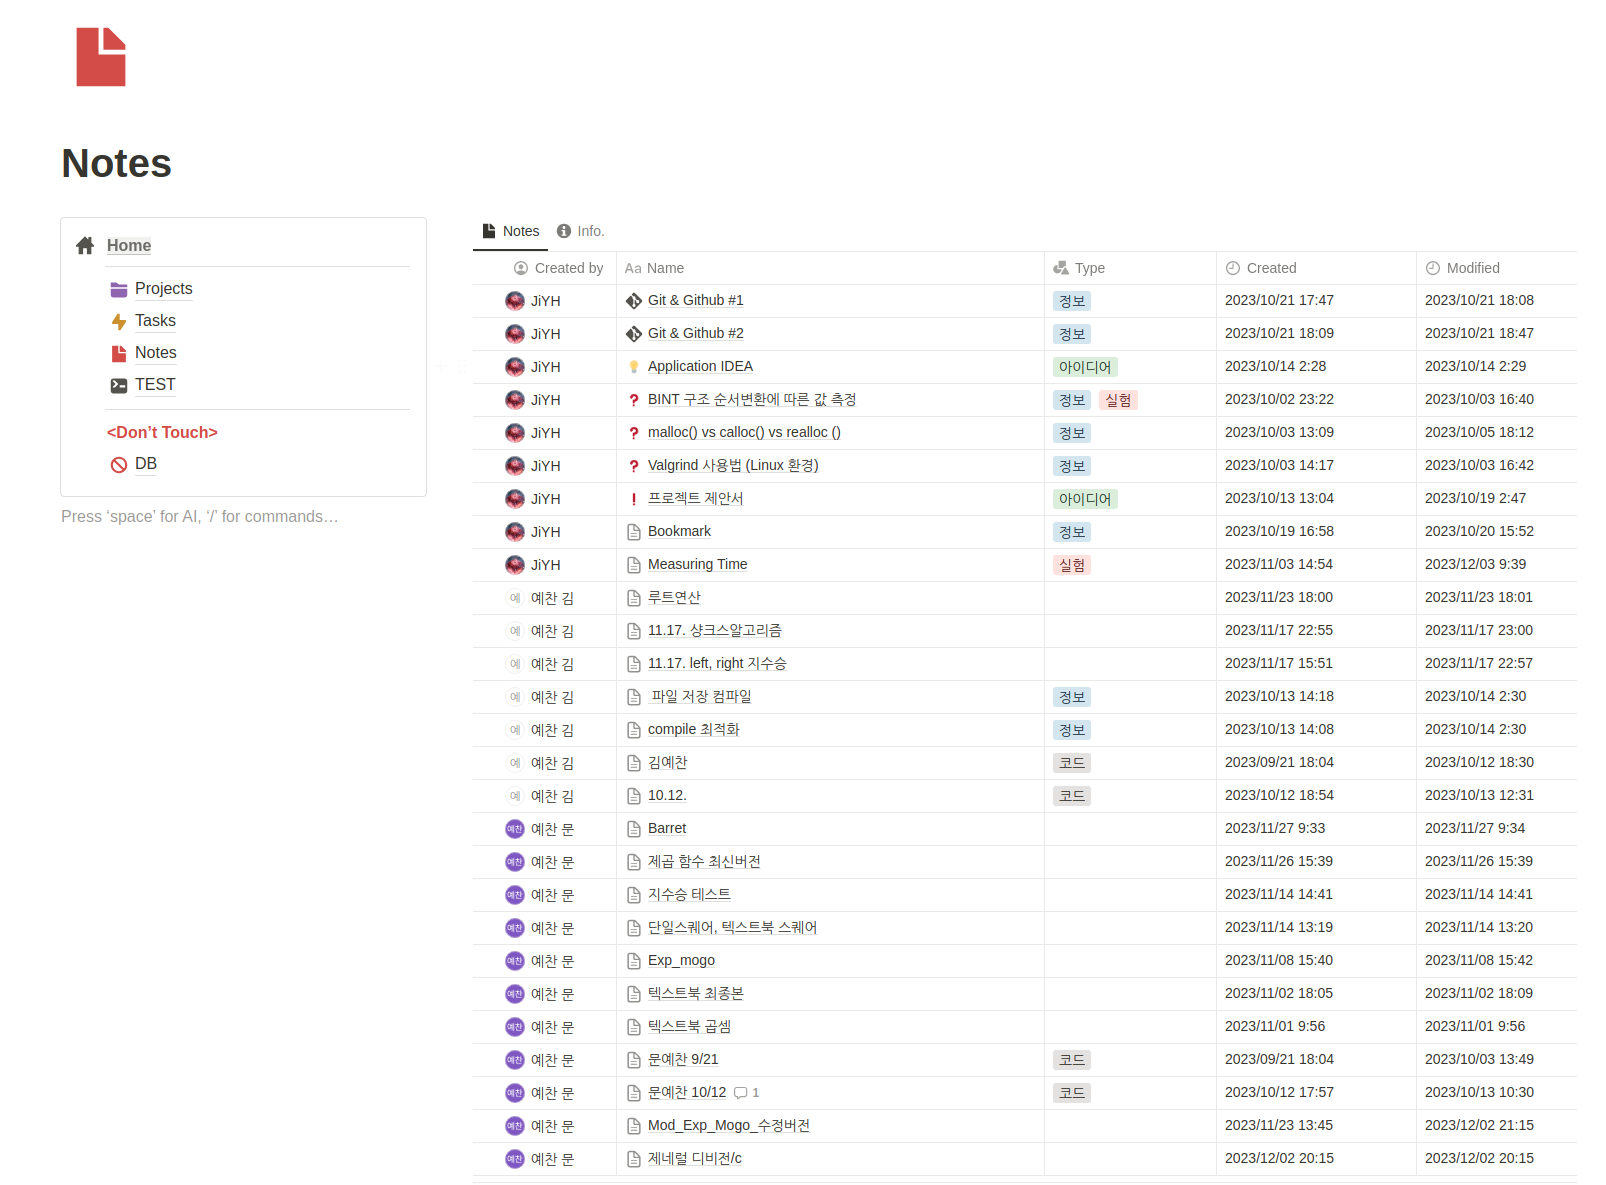
\includegraphics[width=\linewidth,height=.825\textheight]{notion5.png}\\
\end{frame}
\begin{frame}
	\frametitle{II.2 개발 전략 - Notion을 통한 협업}
	\alert{\bf To-Do List와 개발 현황 테이블}\\
	\ \\
	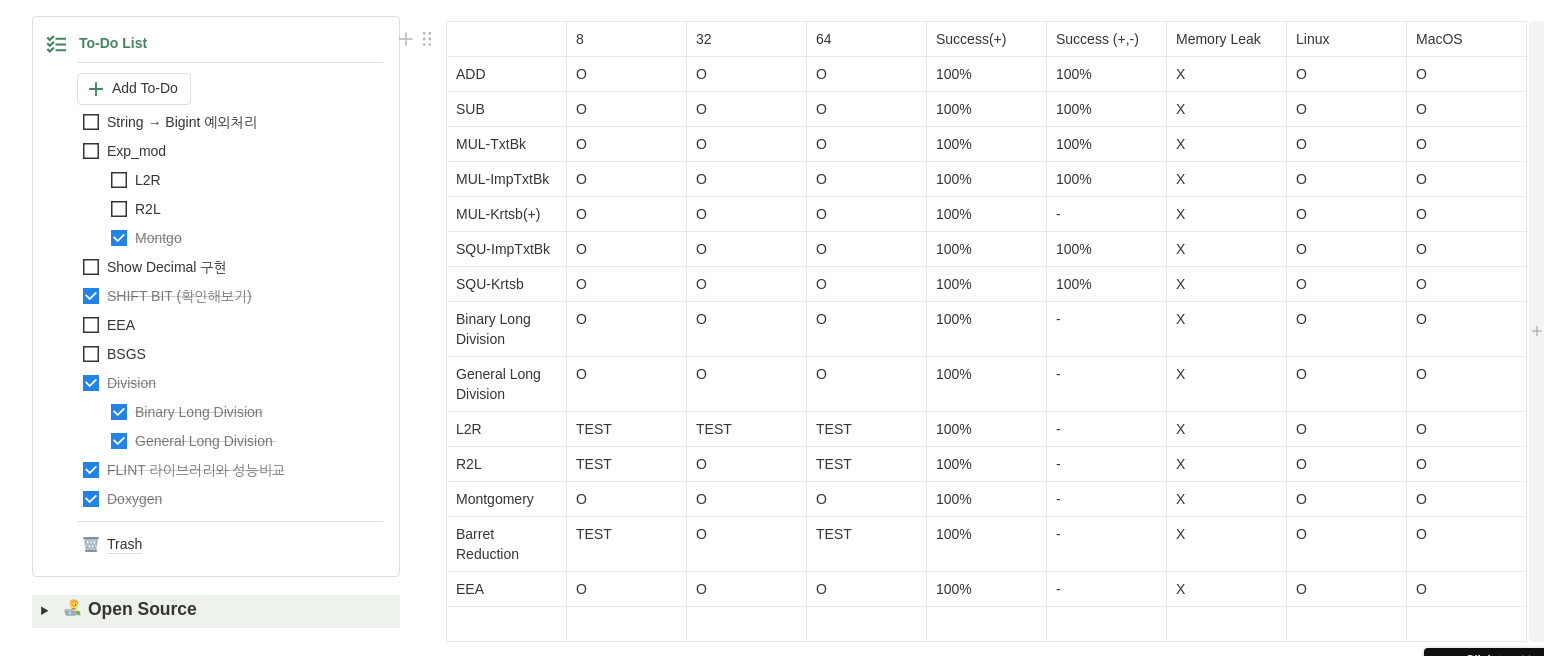
\includegraphics[width=\linewidth,height=.825\textheight]{notion2.png}\\
\end{frame}
\begin{frame}
	\frametitle{II.2 개발 전략 - Notion을 통한 협업}
	\alert{\bf 프로젝트 진행상황 파악 (Board 형)}\\
	\ \\
	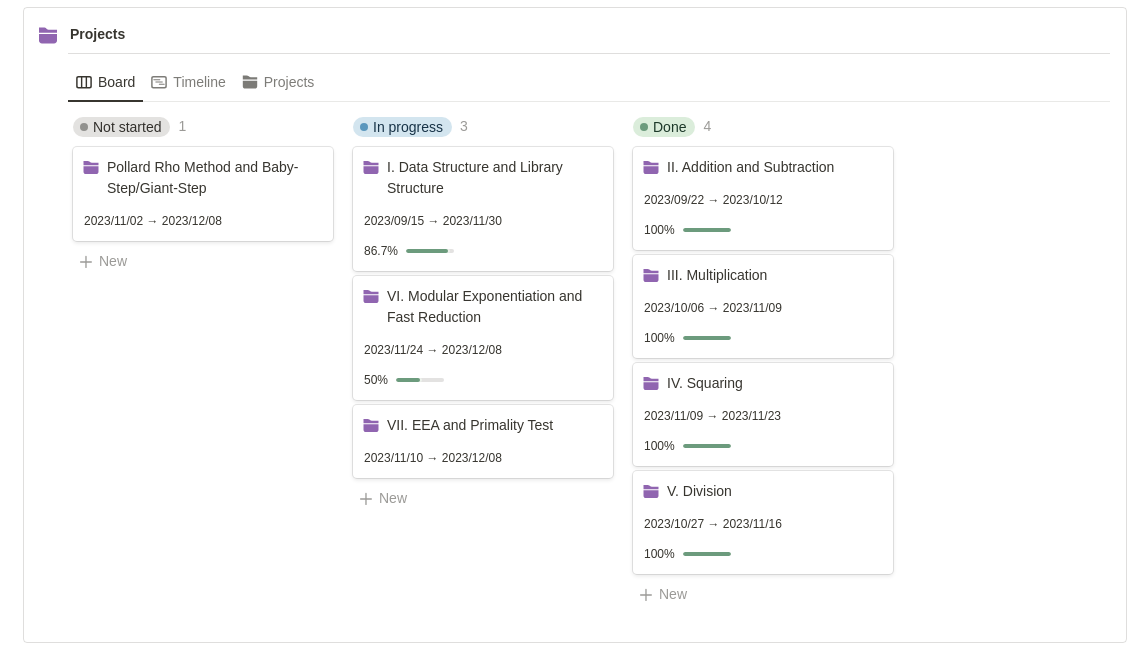
\includegraphics[width=\linewidth,height=.825\textheight]{notion3.png}\\
\end{frame}

\begin{frame}
	\frametitle{II.2 개발 전략 - Notion을 통한 협업}
	\alert{\bf 프로젝트 진행상황 파악 (Timeline 형)}\\
	\ \\
	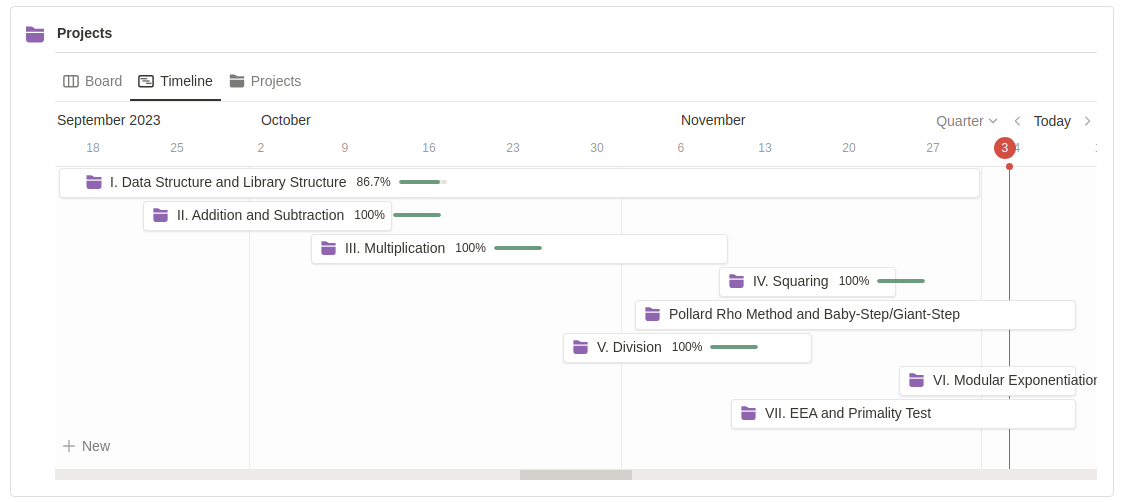
\includegraphics[width=\linewidth,height=.825\textheight]{notion4.png}\\
\end{frame}

\begin{frame}
	\frametitle{II.3 개발 전략 - 개발자 노트 작성}
		\alert{\bf 개발자 노트를 통한 지식 공유}\\
		\ \\
		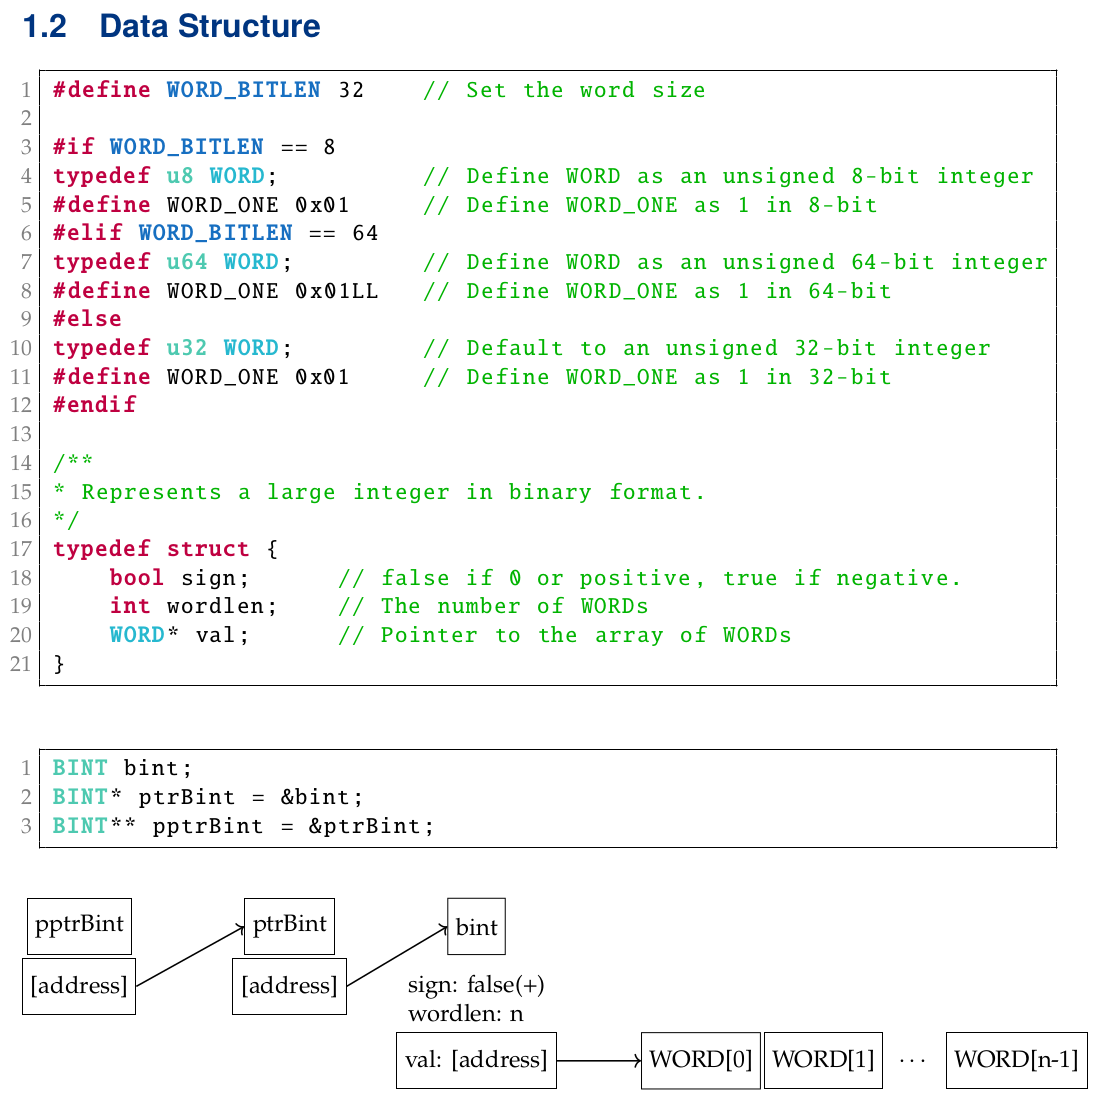
\includegraphics[width=\linewidth,height=.825\textheight]{note1.png}
\end{frame}

\section{III. 라이브러리야, 너의 힘을 보여줘!}
\begin{frame}{IV.1 라이브러리의 필요성}
		\begin{table}[h!]
			\centering
			\begin{tabularx}{\textwidth}{l||X|Xr}
				\toprule
				\multirow{2}{*}{\bf Date}&\textbf{Security}&\multicolumn{2}{c}{\bf Discrete Logarithm}\\
				& \textbf{Strength (bits)}& \textbf{Key (bits)} & \textbf{Group (bits)} \\
				\midrule
				Legacy & 80 & 160 & 1024\\
				2019-2030 & 112 & 224 & 2048\\
				2019-2030 \& beyond & 128 & 256 & 3072\\
				2019-2030 \& beyond & 192 & 384 & 7680\\
				2019-2030 \& beyond & 256 & 512 & 15360\\
				\bottomrule
			\end{tabularx}
			\caption{NIST (2020) \url{https://www.keylength.com/en/4/}}
			\label{tab:c_data_types}
		\end{table}
\end{frame}

\begin{frame}{IV.1 라이브러리의 필요성}
\begin{table}[h!]
	\centering
	\begin{tabularx}{\textwidth}{XX}
		\toprule
		\textbf{Data Type} & \textbf{Size (Bits)} \\
		\midrule
		\texttt{char} & 8 \\
		\texttt{short int} & 16 \\
		\texttt{int} & 32 \\
		\texttt{long int} & 32, 64 (depends on the system) \\
		\texttt{long long int} & 64 \\
		\bottomrule
	\end{tabularx}
	\caption{Basic C language data types and their size constraints.}
	\label{tab:c_data_types}
\end{table}
\end{frame}

\begin{frame}{IV.2 라이브러리 구조}
	\begin{center}
		\begin{tikzpicture}[sibling distance=15em,
			every node/.style = {shape=rectangle, rounded corners,
				draw, align=center}]
			\node {\texttt{config.h}}
			child { node {\texttt{utils.h}} 
				child { node {\texttt{utils.c}} 
					child { node {\texttt{init\_bint()}\\ \texttt{delete\_bint()}\\ $\vdots$} }
				}
				child { node {\texttt{arithmetic.h}}
					child { node {\textcolor{blue}{\bf \texttt{arithmetic.c}}} 
						child { node {\texttt{ADD()}\\ \texttt{SUB()}\\$\vdots$ \\ \texttt{EEA()}} }
					}
					child { node {\texttt{dlp.c} (개발 중)}}
				}
			};
		\end{tikzpicture}
	\end{center}
\end{frame}

\begin{frame}{IV.2 라이브러리 구조}
	\alert{\bf `\texttt{arithmetic.c}' 에서 구현된 함수들 살펴보기}\\
	\begin{itemize}
		\item \texttt{ADD();}
		\item \texttt{SUB();}
		\item \texttt{MUL\_Core\_ImpTxtBk\_xyz();}
		\item \texttt{MUL\_Core\_Krtsb\_xyz();}
		\item \texttt{SQU\_TxtBk\_xz();}
		\item \texttt{SQU\_Krtsb\_xz();}
		\item \texttt{DIV\_Binary\_Long();}
		\item {\texttt{DIV\_Long();}}
		\item \texttt{EXP\_MOD\_L2R();}
		\item \texttt{EXP\_MOD\_R2L();}
		\item \texttt{EXP\_MOD\_Montgomery();}
		\item {\texttt{Barret\_Reduction();}}
		\item \texttt{EEA();}
	\end{itemize}
\end{frame}

\begin{frame}{IV.3 라이브러리 검증 및 테스트}
	\alert{\bf 지원 OS}\\
	\begin{itemize}
		\item Linux
		\item MacOS
	\end{itemize}
	\alert{\bf 메모리 누수}\\
	Linux: \texttt{valgrind --leak-check=full --show-leak-kinds=all}\\
	MacOS: \texttt{leaks}\\
	\begin{center}
		\begin{minipage}{.4\linewidth}
			
\includegraphics[scale=1.5]{lib1.jpeg}
		\end{minipage}
	\begin{minipage}{.55\linewidth}
	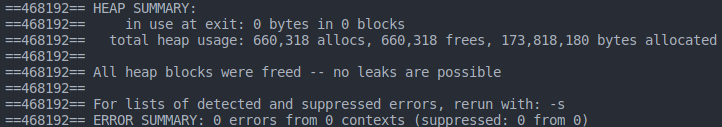
\includegraphics[scale=.25]{lib2.png}\\
	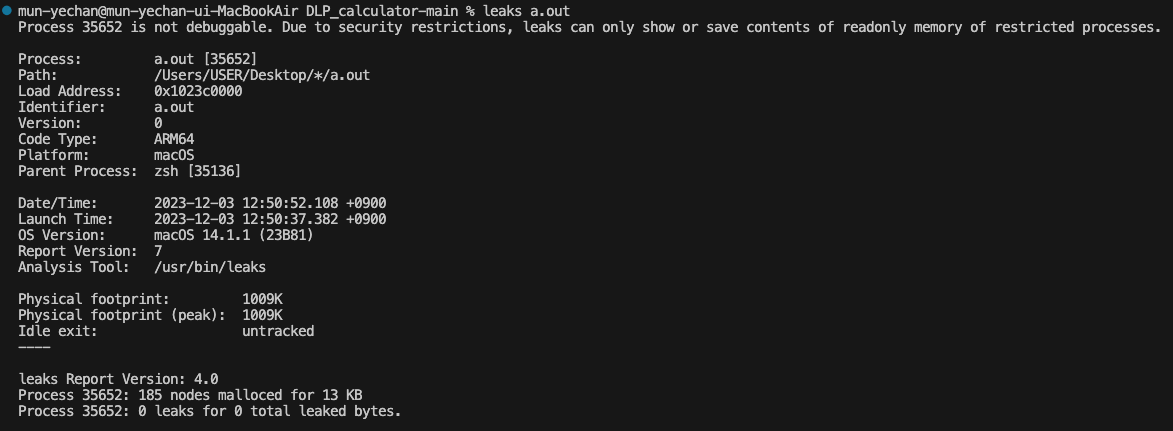
\includegraphics[scale=.15]{lib2_1.png}
\end{minipage}
	\end{center}
\end{frame}

\begin{frame}{IV.3 라이브러리 검증 및 테스트}
	\alert{\bf 정확도 테스트}\\
	\begin{flushleft}
		\begin{minipage}{.8\linewidth}
			구현한 함수가 계산이 잘 되는지 어떻게 확인할까?
		\end{minipage}
		\begin{minipage}{.15\linewidth}
			
\includegraphics[scale=.15]{lib3.jpg}
		\end{minipage}
	\end{flushleft}
	
	\alert{\bf Step 1. 파이썬 코드로 출력}\\
	\begin{center}
		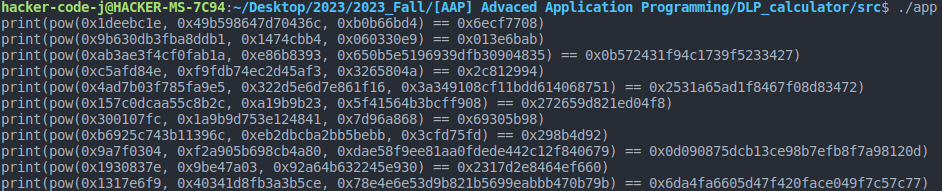
\includegraphics[width=\linewidth]{lib4.png}
	\end{center}
\end{frame}
\begin{frame}{IV.3 라이브러리 검증 및 테스트}
	\alert{\bf Step 2. Makefile을 통한 자동 txt 파일 전환}\\
	\begin{center}
		\begin{minipage}{.45\linewidth}
			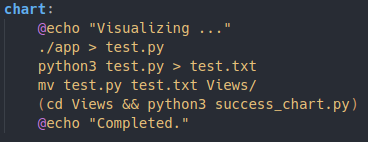
\includegraphics[width=\linewidth]{lib4_2.png}
		\end{minipage}
	\begin{minipage}{.45\linewidth}
	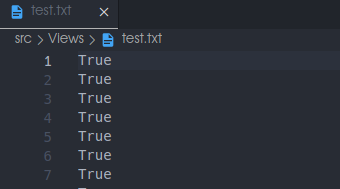
\includegraphics[width=\linewidth]{lib4_3.png}
\end{minipage}
	\end{center}
\end{frame}
\begin{frame}{IV.3 라이브러리 검증 및 테스트}
	\alert{\bf Step 3. 파이썬을 활용해 txt파일을 읽어서 시각화}\\
	\begin{center}
		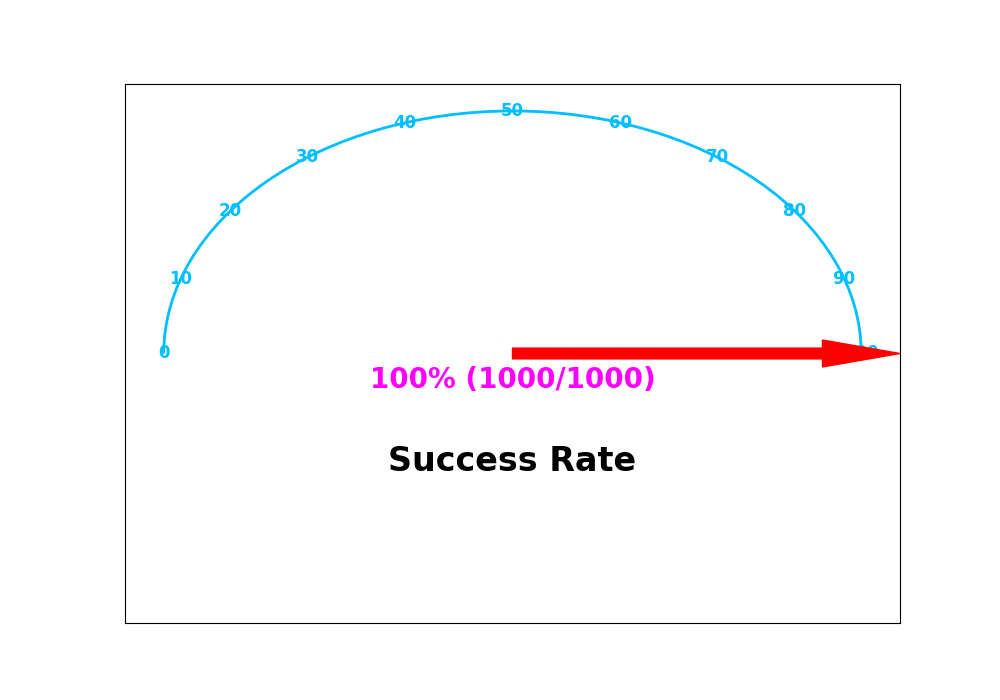
\includegraphics[width=\linewidth]{lib4_4.png}
	\end{center}
\end{frame}
\begin{frame}{IV.4 라이브러리 성능}
	\begin{center}
		라이브러리 성능은 어느정도일까?\\
		\ \\
		
\includegraphics[scale=.5]{lib4_0.png}
	\end{center}
\end{frame}
\begin{frame}{IV.4 라이브러리 성능}
	\alert{\bf 곱셈(TextBook vs Improved TextBook vs Karatsba)}\\
	\begin{center}
		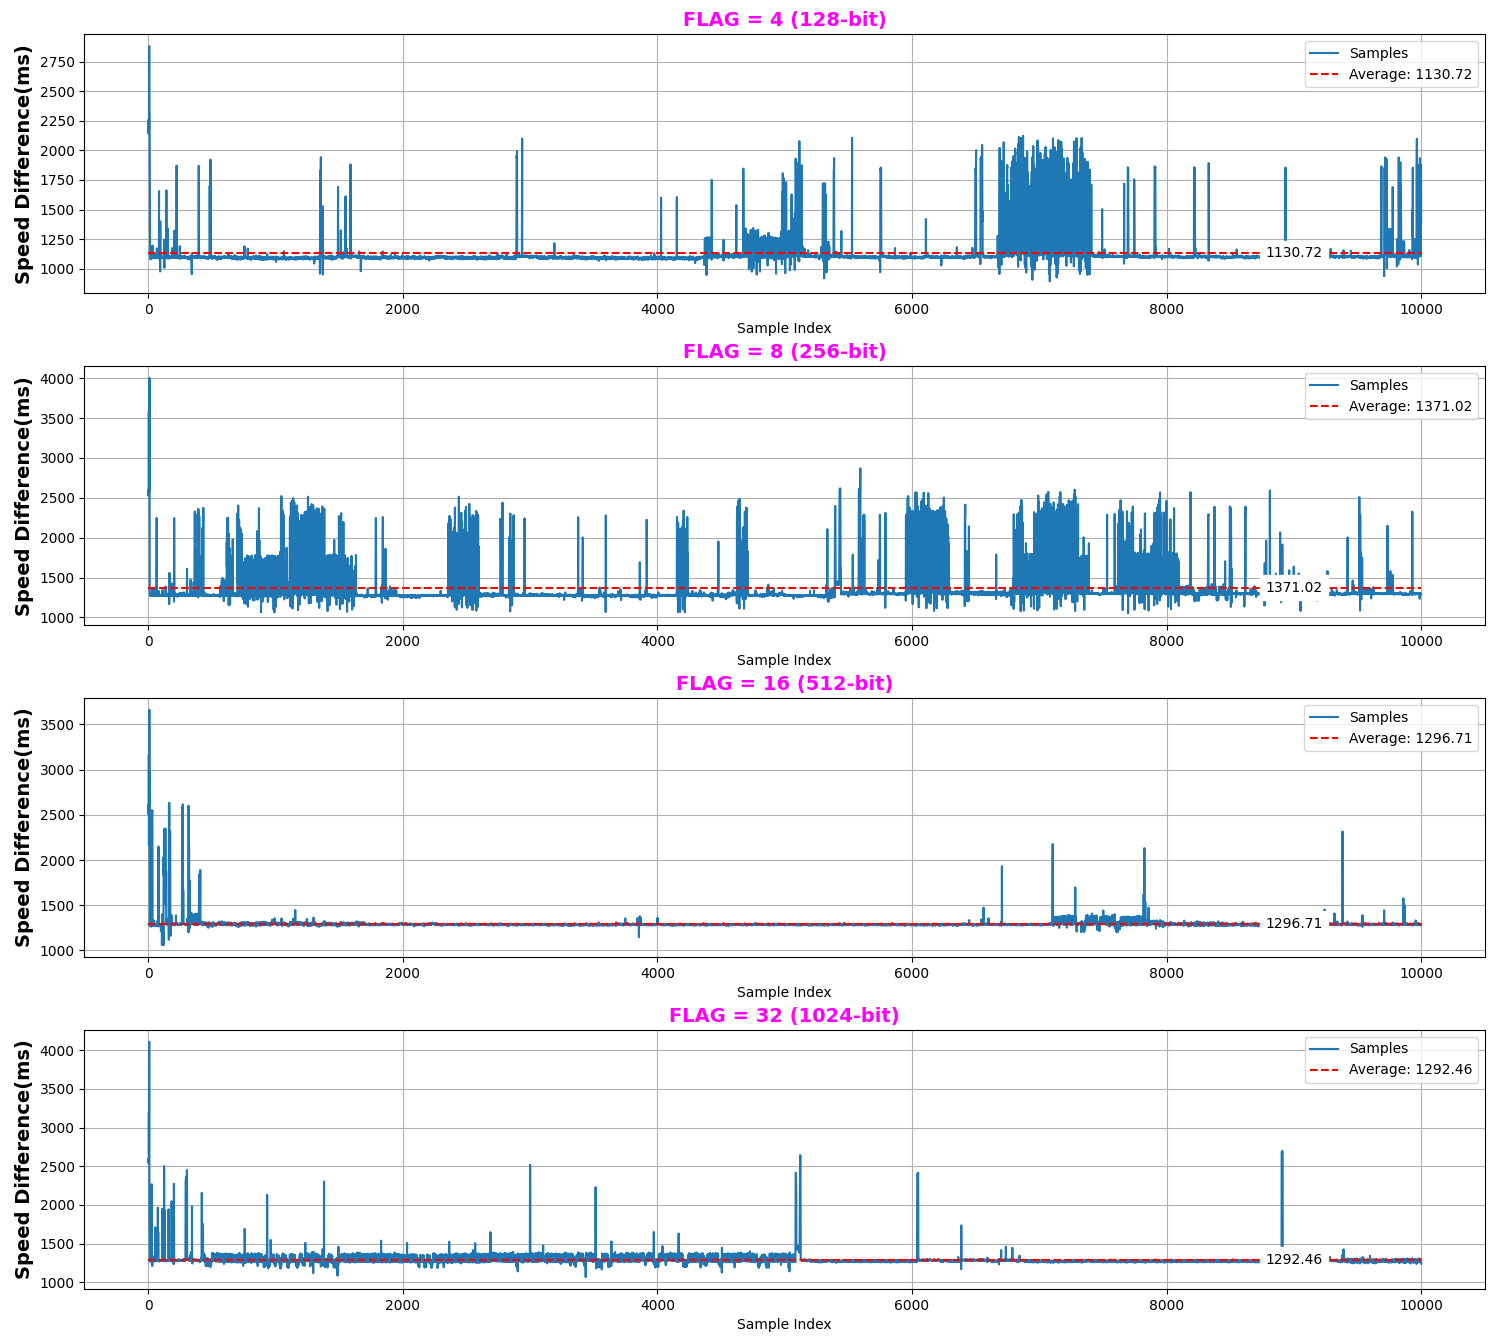
\includegraphics[width=\linewidth,height=.825\textheight]{flag_3072.png}
	\end{center}
\end{frame}
\begin{frame}{IV.4 라이브러리 성능}
	\alert{\bf 곱셈(TextBook vs Improved TextBook vs Karatsba)}\\
	\begin{center}
		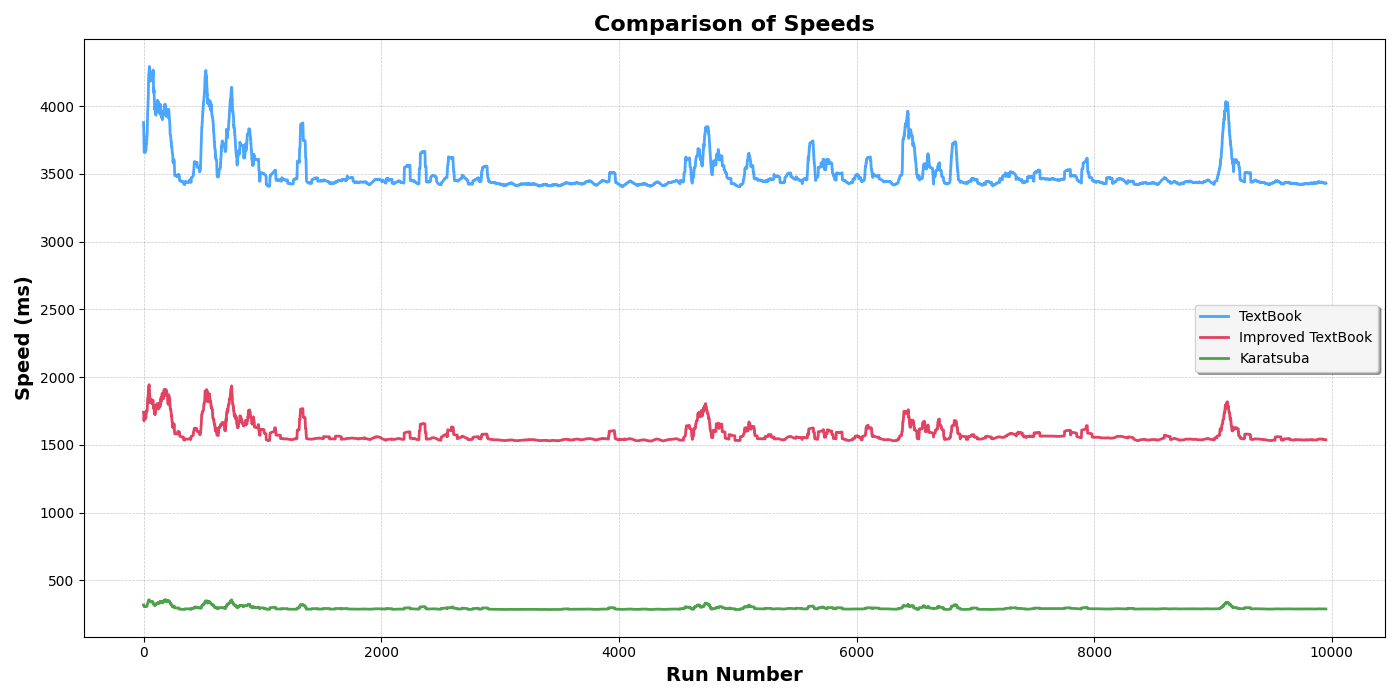
\includegraphics[width=\linewidth,height=.525\textheight]{mul_3072.png}
	\end{center}
	\begin{center}
		\begin{tabularx}{\textwidth}{c||XX}
			\hline
			방식 & 3072-bit (ms) & 상대 속도(s)\\
			\midrule
			\textcolor{blue}{\bf TextBook} & 3339 & 2.356 \\
			\textcolor{red}{\bf Improved TextBook} & 1417 & 1\\
			\textcolor{green}{\bf Karatsuba} & 296 & 0.209\\
			\hline
		\end{tabularx}
	\end{center}
\end{frame}
%\begin{frame}{IV.4 라이브러리 성능}
%	\alert{\bf 나눗셈(Binary Long vs General Long)}\\
%	\begin{center}
%		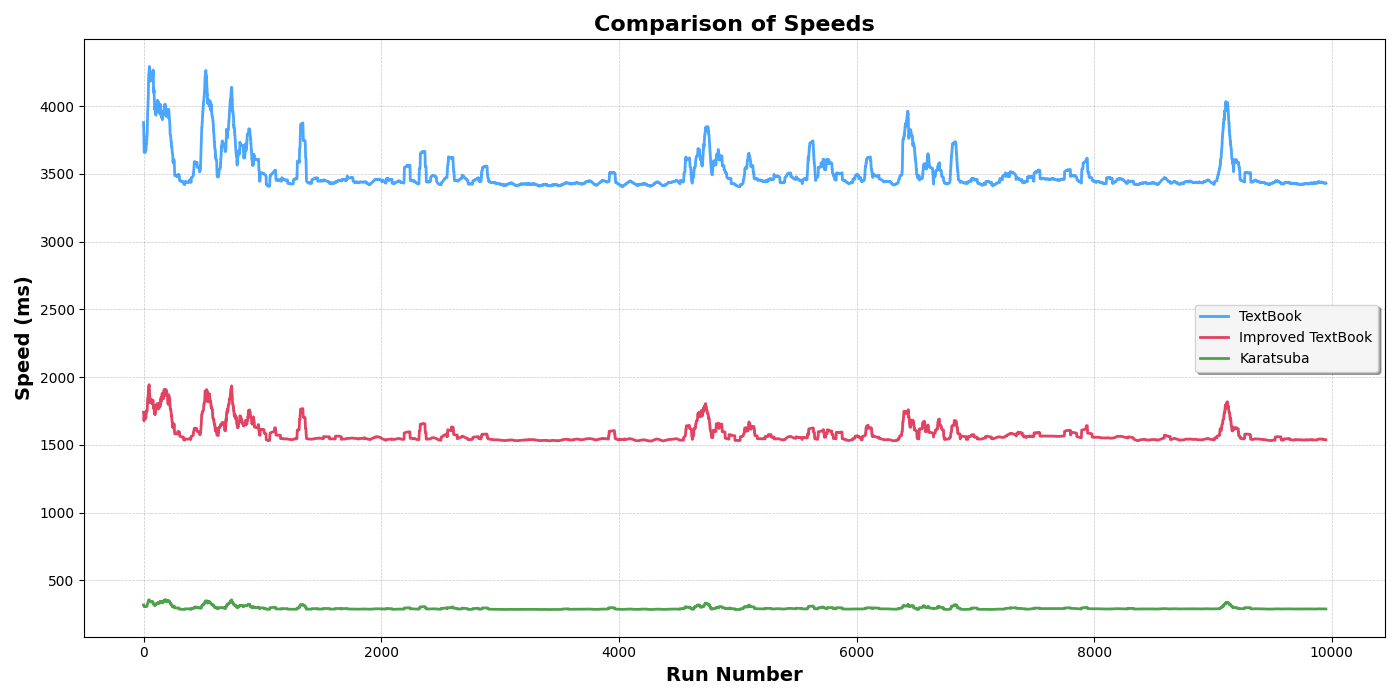
\includegraphics[width=\linewidth,height=.525\textheight]{mul_3072.png}
%	\end{center}
%	\begin{center}
%		\begin{tabularx}{\textwidth}{c||XX}
%			\hline
%			방식 & 3072-bit (ms) & 상대 속도(s)\\
%			\midrule
%			\textcolor{blue}{\bf TextBook} & 3339 & 2.356 \\
%			\textcolor{red}{\bf Improved TextBook} & 1417 & 1\\
%			\textcolor{green}{\bf Karatsuba} & 296 & 0.209\\
%			\hline
%		\end{tabularx}
%	\end{center}
%\end{frame}

\section{IV. 라이브러리의 진가를 보여주지!}

\begin{frame}{IV.1 라이브러리 활용 (개발 진행 중)}
	\begin{center}
		라이브러리 어떻게 활용할까?\\
		\ \\
		
\includegraphics[scale=.3]{lib5.png}
	\end{center}
\end{frame}

\begin{frame}{IV.1 라이브러리 활용 (개발 진행 중)}
	\alert{\bf Baby-step/Giant-step Algorihtm}\\
	\ \\
	\begin{algorithm}[H]
		\KwData{Generator $g$ s.t. $\langle g\rangle = G$ with $|G|=n$. And $h\in G$.}
		\KwResult{The discrete logarithm $x\in\mathbb{Z}_n$ such that $g^x = h$.}
		$m \leftarrow \lfloor\sqrt{n}\rfloor+1$ \tcp*{$m>\sqrt{n}$}
		$BS\gets\set{(i,g^i):i=0,1,\cdots, m-1}$ \tcp*{Baby-step}
		$GS\gets\set{(j, h(g^{-m})^j):i=0,1,\cdots, m-1}$ \tcp*{Giant-step}
		Find $i,j$ such that $g^{i}=h({g^{-m}})^j$\;
		\Return $x\gets mj+i$\;
		\caption{Baby-step/Giant-step Algorithm}
	\end{algorithm}
\end{frame}

\begin{frame}{IV.2 추후 개발 계획}
	\alert{\bf Pollard's $\rho$ Method for DLP}\\
	\begin{center}
		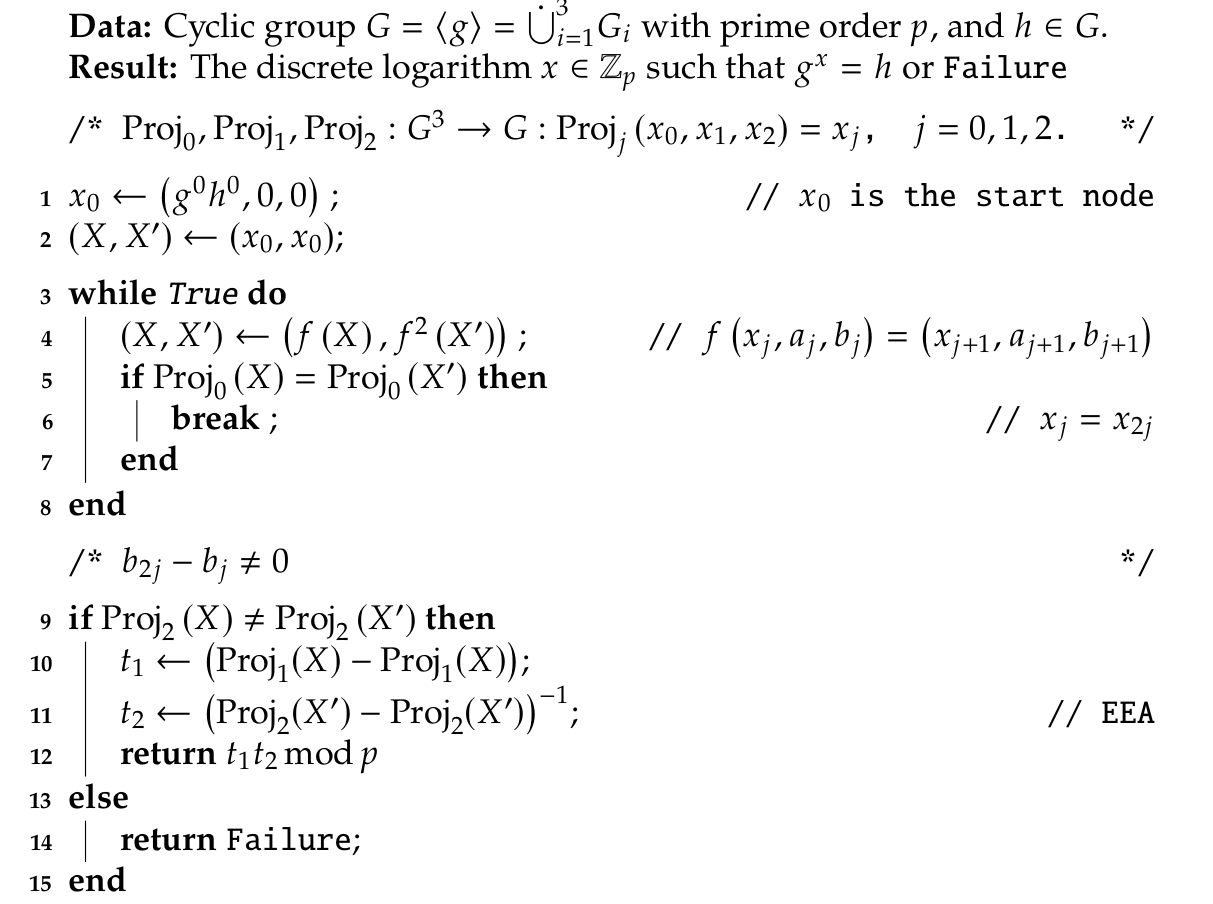
\includegraphics[scale=.225]{rho.png}
	\end{center}
\end{frame}

\section{V. 역시 돈이 최고야!}
\begin{frame}{수익 모델}
	% For a more dynamic slide, use overlays
	\begin{itemize}[<+->]
		\item Key Revenue Stream 1
		\item Key Revenue Stream 2
		% and so on
	\end{itemize}
\end{frame}

\begin{frame}{Revenue Model}
	% For a more dynamic slide, use overlays
	\begin{itemize}[<+->]
		\item Key Revenue Stream 1
		\item Key Revenue Stream 2
		% and so on
	\end{itemize}
\end{frame}

\begin{frame}{Questions?}
	\begin{center}
		
\includegraphics[scale=.35]{end.jpg}
	\end{center}
%	\centering \Large
%	Any Questions?
\end{frame}

\end{document}